%Chapter8
\chapter{System architecture}
\label{Chapter8}
The entire system is based on an acquisition device named Zecg, and a native mobile application on the Android platform. Our focus and main effort were on the developing of the mobile application fulfilling all the requirements. The acquisition device was instead developed and designed by Crespi Alessandro and Ulisse Pizzagalli during their thesis work at the Politecnico of Milan.
\section{Acquisition device}
Zecg is composed by the following different modules:
\begin{enumerate}
	\item OVP: used to protect the patient from high voltage or voltage leakage.
	\item LFP EMI Filter: anti-aliasing RC filter used to remove noises due to high frequencies.
	\item RLD: Active electrode driver for the right leg
	\item WCT: Derivator used to compute the precordials (Wilson Central Terminator)
	\item PGA: 8 gain amplifier with programmable inputs
	\item ADC: 8 analog-digital 16 bit 8KSa/s converter.
	\item MCU: microcontroller
	\item Bluetooth: bluetooth module for data transmission
	\item Power MGMT: to manage battery recharge and stabilizer
\end{enumerate}
\begin{figure}[ht!]
	\centering
	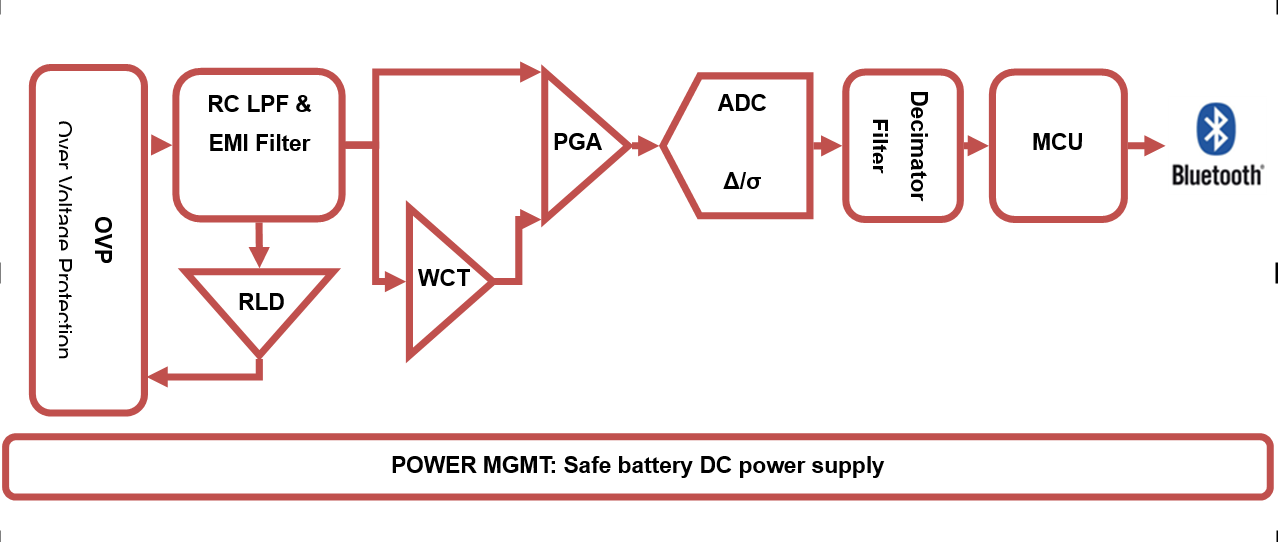
\includegraphics[width=110mm]{figures/ch8/1.png}
	\caption{ZEcg device block diagram including all the modules components.}
	\label{fig8.1}
\end{figure}
The core component is the Texas Instrument system on chip ADS1198. This chip has 8 input bipolar channels, representing the 8 clinical leads.\\
The channels 1 and 2 produce the lead I and lead II. Channel 1 measures the potential difference between the electrode RA(-) and the electrode LA(+), the channel 2 the difference between RA(-) and LL(+). Lead III and the augmented leads are obtained from a combination of lead I and lead II at software level.\\
V1, V2,...,V6 are computed as difference between the respective electrode and the signal related to the negative value of the WCT (Wilson Central Terminator).\\
The WCT signal comes from the average between RA, LA and LL and it's connected to the channels 3,4,5,6,7,8.
\begin{figure}[ht!]
	\centering
	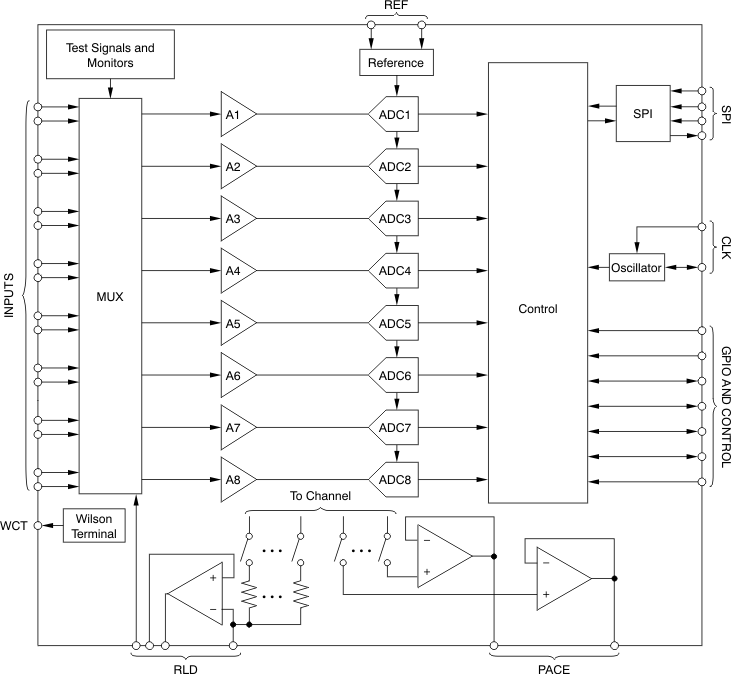
\includegraphics[width=120mm]{figures/ch8/2.png}
	\caption{ADS1198 functional diagram showing the 8 channels representing the 8 leads used during the ECG record acquisition.}
	\label{fig8.2}
\end{figure}
Each channel is amplified using a programmable gain (PGA) and a CMRR, before being converted into digital. For more details about the entire device architecture we invite you to read the thesis of our colleagues Crespi Alessandro and Ulisse Pizzagalli\cite{ref22} who designed and developed zecg.
\subsection{Mobile app}
The mobile application we developed for this thesis work was implemented having in mind all the user best interface design principles and the best practice starting from the planning and design phase to the final  coding phase. As this application was designed for Android OS, we strictly followed Google specific standards and procedures.\\
We made use of Android Studio as IDE (strongly suggested by Google as main IDE to develop Android native applications). Starting from 2013 the development of native Android application moved from Eclipse + Android Plugin to Android Studio. The entire project building system has changed and moved to use the Gradle  building system\cite{ref23}. 
The entire process during project building to compilation can be resumed in the following image:
\begin{figure}[ht!]
	\centering
	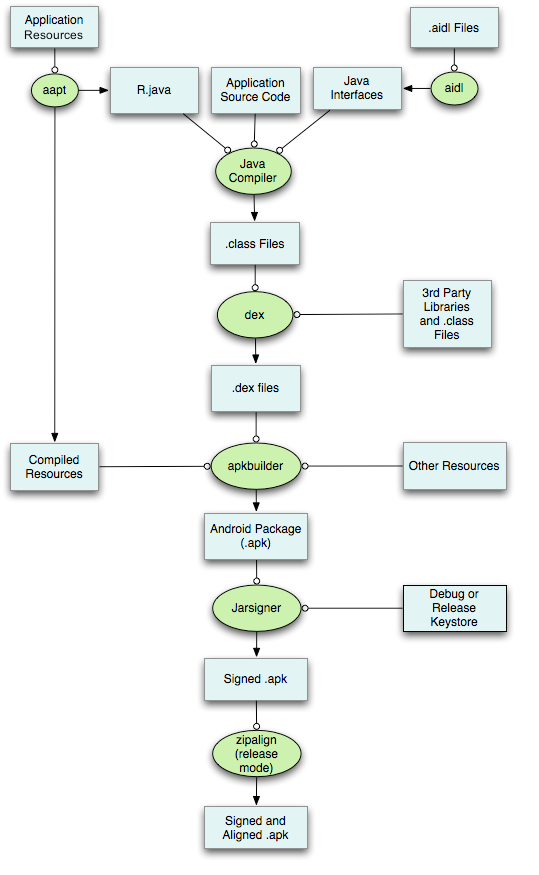
\includegraphics[width=90mm]{figures/ch8/3.png}
	\caption{Android Build system process. How and which component are involved during an android application build and compilation.}
	\label{fig8.3}
\end{figure}
The most important steps along the building process are:
\begin{enumerate}
	\item The Android Asset Packaging Tool (aapt) takes the application resource files, such as AndroidManifest.xml file and the XML files for the Activities, and compiles them. A R.java  file is produced so that all the resources can be easly accessed within your application.
	\item The aidl tool converts any .aidl interfaces into Java interfaces.
	\item The Java compiler will compile the R.java and .aidl files generating the .class files.
	\item The Dex tool will convert the .class files to Dalvik bytecode. Any 3rd libraries and .class files included in the project build will be also converted into .dex files so that they can be later packed into the final .apk.
	\item All non-compiled resources(such as images), compiled resources, and the .dex files  are sent to the apkbuilder tool that will output the .apk file.
	\item Once the .apk is built, it must be signed with either a debug or release key before it can be installed to a device.
	\item To reduce the size of the .apk and to decrease the memory usage for releasing mode the zipalign tool is launched.
\end{enumerate}
We split the application functionalities into different packages. 
\begin{figure}[ht!]
	\centering
	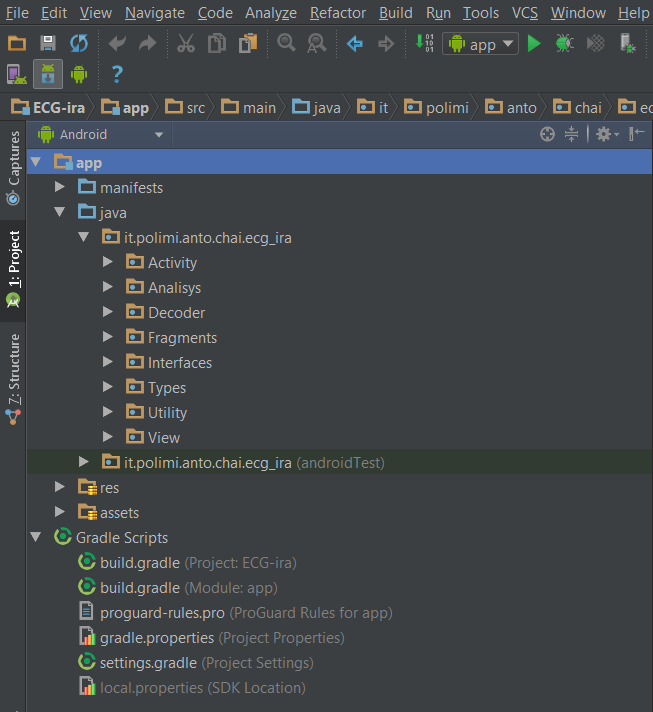
\includegraphics[width=90mm]{figures/ch8/4.png}
	\caption{ECG-ira project structure and packages inside Android Studio IDE.}
	\label{fig8.4}
\end{figure}
The packages content are divided as follow:
\begin{itemize}
	\item Activity: it contains all the Activity used inside the Application.
    \item Analysis: All the java classes used for the analysis of the ECG records; they include the Neural Network, the QRSDetector, the PWaveDetector and some signal Filters implementations.
	\item Decoder:  this package contains the java classes in charge to decode and parse the .hea and .dat files.
	\item Fragments: contains some fragments used inside the application, for example  the ones used to show the chronograms (Istogram, Tacogram, ST graphs).
	\item Interfaces: all interfaces declarations to abstract the specific application behaviour with more general one.
	\item Utility: some utility class such as the in application FileManager.java class, and the Adapters used within the application (for example to show ListViews or RecycleViews).
	\item View: it contains all the classes working directly on the View and the custom view themselves such as the View used to show the ECG grid.
\end{itemize}
The key points of this application are based on three main concepts:
\begin{itemize}
	\item Code reuse and maintainability
	\item Maximize performance depending on the device constraints (cpu, memory, storage capacity)
	\item Usability in term of interface and interaction
\end{itemize}
\subsubsection{Code reuse and maintainability}
The most important classes representing the core of the application functionalities are all abstracted through interfaces or in case of the classes related to the View through a set of parameters. This makes the application highly customizable and easily to extend. For example if in a next future there will be a new ECG data format, it can be possible to give the app the capability to read and parse such a format just by implementing the interfaces and writing the specific code to parse such a new data format.\\
A concrete example is given in our code by observing that both the MITDatReader and the ZEcgDatReader extends the abstract class DatReader, so the next format reader has just to extend it as well. We know that MIT-BIH format is completely different from the ZEcg format, that why specific code to parse the file content to extract the signal is mandatory.\\
Any new format reader has just to override the method:
\begin{lstlisting}
public void readAndAddSample(int numOfSample, int addPosition) {
}
\end{lstlisting}
More concrete details about the effective implementation will be exploited later on in the next chapters.
\subsubsection{Maximize performance depending on the device constraints}
We do well know about the great number of constraints due to the huge number of different devices with different hardware on. We decide to make our application available starting from Android API 16 (the minimum sdk API recommended by Google to support).  To overcome the problem of the difference devices and Android OS version starting from Jelly Bean (API 16) we took maximum advantages from the device hardware by splitting the thread jobs in between the maximum number of cores available. In the class CpuInfoExtractor we discover the hardware capabilities (number of cores) and according to it we split the calculus between a certain number of threads. More the cores, more the threads we can take advantage of.\\
From an interface point of view instead, we are forced  to depend on the density of pixel of the device screen and its size, but at the same time to accomplish our requirements related to achieve a perfect grid of squares of centimeters. We found a way to always achieve the same dimensions of square independently by the screen size of the devices by retrieving and taking in account the display exact pixels per inch size in the X dimension. Then, we computed the number of pixels needed to achieve the right sizing.  In this way, we solved the problem of having same dimensions and so metrics on different devices. On the other hand, if this method is quite functional and device independent, on devices with different screen size (width for example) the number of grid cells may vary from just a few on small screen, to many of them on tablets. This is a direct consequence due to the difference in number of pixels and the pixels size itself (some are square, most of them are rectangle).\\

\subsubsection{ Usability in term of interface and interaction}
One mobile application is usable if it does what the user expects it to do when interacting with it.\\
We followed all Google guidelines in term of user experience using native view and patterns. We took advantage of the last API features, such as RecycleViews instead of the old classic ListViews. We made use of the button ripple effects available starting from Lollipop (Android API 21), but at the same time we provided to the older Android OS version the selector effect which still gives a nice response to the user interaction with command and buttons. We made use of the typical android Preference Settings so familiar to Android users and most important we always inform the user about the operations going on so he never feels lost inside the application.